\begin{center}
\begin{figure}
\centering
%\resizebox{8cm}{4cm}{
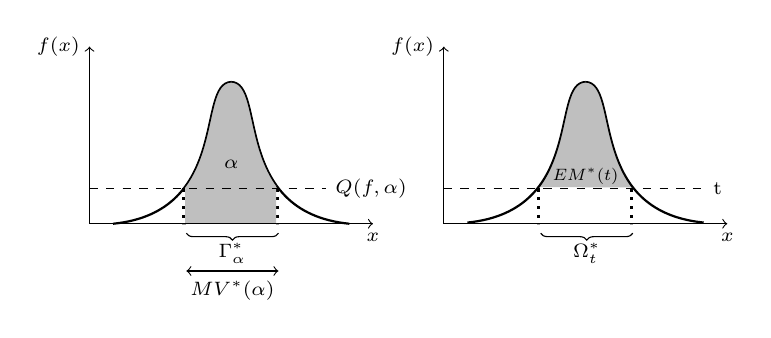
\begin{tikzpicture}[scale=1.5]

\draw[->](7.8,0)--(10.2,0) node[below]{\scriptsize $x$};
\draw[->](7.8,0)--(7.8,1.5) node[left]{\scriptsize $f(x)$}; 
\draw [thick] (8,0) ..controls +(1,0.1) and +(-0.3,-0.01).. (9,1.2);
\draw [thick] (9,1.2) ..controls +(0.3,-0.01) and +(-1,0.1).. (10,0);

\draw[dotted,very thick](8.60,0.3)--(8.60,0) node[right]{};
\draw[dotted,very thick](9.39,0.3)--(9.39,0) node[right]{};

%\draw (8,0.3)--(10,0.3)--(10,1.5)--(8,1.5)--(8,0.3); dessine 4 segments correspondant au 4 points

%hachurage :
\begin{scope} 
\clip (8.61,0)--(9.38,0)--(9.38,1.5)--(8.61,1.5)--(8.61,0) ; %tout ce qui est dans begin{scope} se limitera au rectangle

\path[draw,fill=lightgray] (8,0) ..controls +(1,0.1) and +(-0.3,-0.01).. (9,1.2)--
(9,1.2) ..controls +(0.3,-0.01) and +(-1,0.1).. (10,0)--
(8,0)--(10,0) --cycle;
\end{scope}

\draw[dashed](7.8,0.3)--(9.8,0.3) node[right]{\scriptsize $Q(f,\alpha)$};

%accolade :
\draw[decorate,decoration={brace}]
(9.4,-0.08)--(8.62,-0.08) node[below,pos=0.5] {\scriptsize $\Gamma_\alpha^*$};

\draw[<->]
(9.4,-0.4)--(8.62,-0.4) node[below,pos=0.5] {\scriptsize $MV^*(\alpha)$};



\draw (9,0.5) node[thick]{\scriptsize $\alpha$} ;
%\draw (8.8,-0.8) node[thick]{Figure 1: MV curve} ;

\draw[->](10.8,0)--(13.2,0) node[below]{\scriptsize $x$};
\draw[->](10.8,0)--(10.8,1.5) node[left]{\scriptsize $f(x)$}; 
\draw [thick] (11,0.01) ..controls +(1,0.1) and +(-0.3,-0.01).. (12,1.2);
\draw [thick] (12,1.2) ..controls +(0.3,-0.01) and +(-1,0.1).. (13,0.01);
\draw[dashed](10.8,0.3)--(13,0.3) node[right]{\scriptsize t};
\draw[dotted,very thick](11.60,0.3)--(11.60,0) node[right]{};
\draw[dotted,very thick](12.39,0.3)--(12.39,0) node[right]{};

%\draw (8,0.3)--(10,0.3)--(10,1.5)--(8,1.5)--(8,0.3); dessine 4 segments correspondant au 4 points

%hachurage :
\begin{scope} 
\clip (11,0.31)--(13,0.308)--(13,1.5)--(11,1.5)--(11,0.308) ; %tout ce qui est dans begin{scope} se limitera au rectangle (8,0.3)--(10,0.3)--(10,1.5)--(8,1.5)--(8,0.3)
\path[draw,fill=lightgray] (11,0) ..controls +(1,0.1) and +(-0.3,-0.01).. (12,1.2)--
(12,1.2) ..controls +(0.3,-0.01) and +(-1,0.1).. (13,0)--
(11,0.3)--(13,0.3) --cycle;
\end{scope}

%accolade :
\draw[decorate,decoration={brace}]
(12.4,-0.08)--(11.62,-0.08) node[below,pos=0.5] {\scriptsize  $\Omega_t^*$};

\draw (12,0.4) node[scale=0.85]{\scriptsize $EM^*(t)$} ;
\draw (11.8,-0.5) node[thick]{ } ;
\end{tikzpicture}
%}
\caption{Comparison between $MV^*(\alpha)$ and $EM^*(t)$}
\label{aistat:MVcurve}
\end{figure}
\end{center}
